\section{Case study \#3: Recomputing non-CS experiments}
\label{s:group3}

In this case study we focus on the issues relevant to research reproducibility that are potentially 
  unique to non-CS computational research.
The discussion is based on experience gained while packaging three computational experiments 
  into recomputable virtual machines.
The papers on which the discussion is based 
  deal with urban planning~\cite{danielpaper}, solar
  physics~\cite{bareford2010nanoflare}, and atmospheric
  physics~\cite{arabas2013libcloud},
  although the discussion is likely relevant to other non-CS domains. One of the
  authors of each paper was involved in this case study.

\subsection{Methodology}

Our aim was to offer potential readers (or reviewers) of the papers in question, 
  the opportunity to reproduce the figures presented in the papers, 
  to inspect the code, and to possibly test behaviour of the programs with other parameters.
To offer it all within a ready-to-use environment, we have used the Vagrant
tool\footnote{\url{https://www.vagrantup.com/}}
to
  construct a single virtual machine with all needed software and its dependencies installed.
The virtual machine was based on the Debian Sid GNU/Linux distribution.

\subsection{Results}
\subsubsection*{Experiment 1: Urban Planning}

For the first paper, we tried to recompute parts of Table~6 of
\cite{danielpaper}, in which the punctuality of a bus service in Edinburgh is
evaluated using statistical methods. Table~6 contains confidence intervals that
are constructed using a piece of software written in Java. It is possible to
compile the source code after installing a Java Software Development Kit on the
virtual machine. The software uses the SSJ library for Stochastic
Simulation\footnote{\url{http://simul.iro.umontreal.ca/ssj-2/indexe.html}},
which had to be downloaded from the Internet. After that, we were able to run
the code.

We encountered legal obstacles in the following two areas.
\begin{itemize} 
\item Code-related: the software was developed as part of the EU project
QUANTICOL\footnote{\url{http://blog.inf.ed.ac.uk/quanticol/}}, which is funded by the European Commission as part of its 7th
Framework programme. In the General Conditions part of the project's grant
agreement, it is stated that the IP rights are awarded to the beneficiary, which
in this case is the University of Edinburgh. In turn, the University of
Edinburgh has issued a position statement on intellectual property
rights\footnote{\url{http://www.research-innovation.ed.ac.uk/Portals/0/Documents/University-of-Edinburgh-Position-Statement-on-Intellectual-Property_December2011.pdf}} in which it stated that it ``\emph{is the policy of the University of Edinburgh to develop University research capabilities and to assess, develop and promote the transfer of Edinburgh's technology and ideas for society's use and benefit.}'' Still, publication of the code would need to be checked with a supervisor.
\item Data-related: the code uses a dataset based on bus location measurements provided to us by Lothian Buses. We would need their permission to put this dataset in the public domain.
\end{itemize}
The use of the SSJ package is not an obstacle because it is released under the GPL licence from GNU.

The resulting virtual machine contains the Java source files, allowing
researchers with knowledge of Java to analyse the correctness of the programme.
However, the code is not documented and may be hard to read. Specifically,
parameters are hard-coded and no interpretation is given of the produced
numbers and \LaTeX\ code.

The output of the Java code is displayed in Table~\ref{tab: z bootstrapped cis}.

\newcommand{\vtwo}[2]{$\left[\begin{array}{l} #1, \\ #2 \end{array}\right]$}
\newcommand{\exr}[1]{\cdot$10$^{#1}}
\newcommand{\hpi}[1]{\hat{\pi}_z(#1)}
\newcommand{\hpic}[1]{\multicolumn{1}{c}{$\hpi{#1}$}}
\newcommand{\hpicl}[1]{\multicolumn{1}{|c}{$\hpi{#1}$}}
\newcommand{\hpicr}[1]{\multicolumn{1}{c|}{$\hpi{#1}$}}

\def\arraystretch{1.2}
\setlength{\tabcolsep}{1pt}
%
\begin{table}[htbp]
\centering
\begin{tabular}{| c c c c c  |} \hline 
 \hpicl{5} & \hpic{6} & \hpic{7} & \hpic{8} & \hpicr{9} \\
 \vtwo{0}{0}&\vtwo{2.875\exr{-4}}{4.253\exr{-4}}&\vtwo{0.434}{0.485}&\vtwo{0.513}{0.566}&\vtwo{0.0}{0.0}\\[10pt]
\hline
\end{tabular}
\caption{A reproduction of the first row of Table 6 of \cite{danielpaper}, which contains confidence interval for estimates of $\pi_z(k)$. For each $k$, $\pi_z(k)$ denotes the probability that, upon arrival to the bus stop near Edinburgh airport, $k$ arrivals of buses of Route~100 are observed in the next hour.}
\label{tab: z bootstrapped cis}
\end{table}
\def\arraystretch{1.5}


\subsubsection*{Experiment 2: Solar Physics}

%At the start of the recomputation exercise it was judged that the results
%presented in \cite{bareford2010nanoflare} would be the easiest (of the three
%publications outside of computer science) to reproduce. The underlying code is
%serial in nature and not tied to specific hardware or operating system platform. 

The work discussed in~\cite{bareford2010nanoflare} concerns the energy released
from an idealised cylindrical magnetic field when it becomes unstable and
subsequently relaxes to a simpler state. Initially, a field (or loop) starts in
a stable configuration and is then taken on a random walk through a known two
dimensional region of stability, see \mbox{Figure 3} of the aforementioned
publication. When the field crosses the boundary of this region (i.e.\ the threshold for instability), an energy release is determined and the field is moved to simpler stable configuration. 

When this process is repeated many times, the results can be expressed as energy distributions, see Figure~14 of~\cite{bareford2010nanoflare}, which shows the energy releases for $10^5$ relaxations involving a variety of loop lifetimes. We decided to focus on reproducing only this figure. The individual plots were taken from the results produced by a C++ code called Taylor Relaxation of Loop Ensembles, or TRoLE for short, that automates the process described above.

The TRoLE code was written when the first author of~\cite{bareford2010nanoflare}
was a postgraduate at the University of Manchester. It was necessary therefore
to check the IP policy for this
institution.\footnote{\url{http://documents.manchester.ac.uk/DocuInfo.aspx?DocID=487}}
Section~3.2 of this policy states that the ``\emph{...ownership of IP created by
a Student, who is not an employee of the University, is with the Student.}'',
which we took to mean that the first author was free to place the code in a
publicly available
repository.\footnote{\url{https://github.com/mbareford/trole}}

The next issue concerned a technical matter: the code uses
a proprietary numerical algorithms library
(NAG),\footnote{\url{http://www.nag.co.uk/numeric/CL/CLdescription.asp}} the
licence for which had expired. Fortunately, there is an open source alternative,
the GNU Scientific Library
(GSL).\footnote{\url{http://www.gnu.org/software/gsl/}} The TRoLE code was updated such that all NAG calls were replaced with the GSL alternative. 

%After the code was recompiled and linked with the GSL libraries, it was ready to
%run the simulation of $10^5$ relaxation events. Alas, the code could at first
%only simulate a fraction of this total (146 events): the code reported that it
%had reached a point on the instability threshold for which a stable (relaxed)
%configuration could not be calculated. The relaxed state is determined by
%ensuring that certain properties are conserved (i.e.\ the property values match
%those calculated for the unstable state)---this is essentially a root finding
%exercise. Further investigation revealed that the magnetic field profiles were
%being calculated incorrectly for a wide range of threshold states. The cause
%concerned incorrect substitutions for the NAG Bessel functions. For example, the
%NAG routine, nag\_bessel\_j0() is the call for a regular cylindrical Bessel
%function, whereas, what looks like the equivalent in GSL, gsl\_bessel\_j0(), is
%actually the routine for a regular \textit{spherical} Bessel function. All that
%was required to call the correct routine was to capitalise the last letter,
%i.e.\ gsl\_bessel\_J0().
% 
%The magnetic field that describes every possible loop configuration is defined in terms of cylindrical 
%  Bessel functions: hence, an error here will have dramatic consequences for the results produced by the 
%  TRoLE code. 
%Once these function calls were corrected, the recomputation was successful. 

Figure \ref{fig_recomp_grp3_exp2} shows two of the recomputed plots, the published energy distributions 
  \cite{bareford2010nanoflare} are given in blue.
\begin{figure}
\begin{minipage}{\linewidth} 
  %\vspace{-10pt}
  \center
  %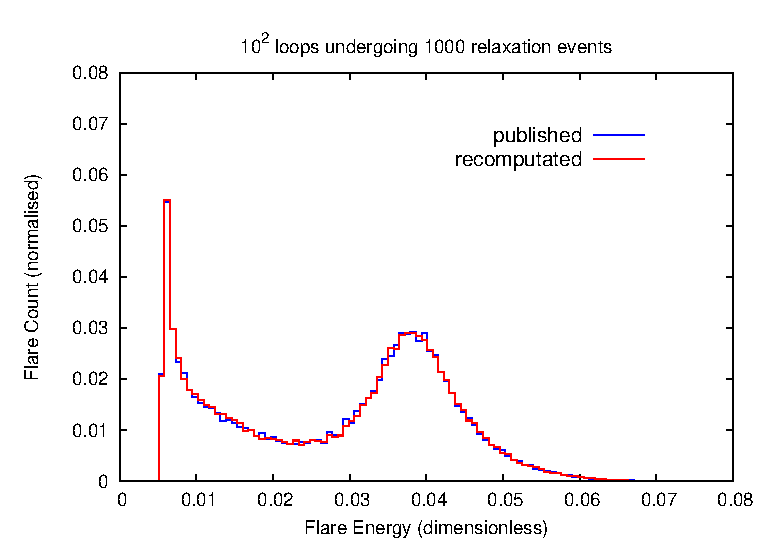
\includegraphics{../Group_3/wrpf_rx10e5_lle3}
  %\vspace{5pt}
  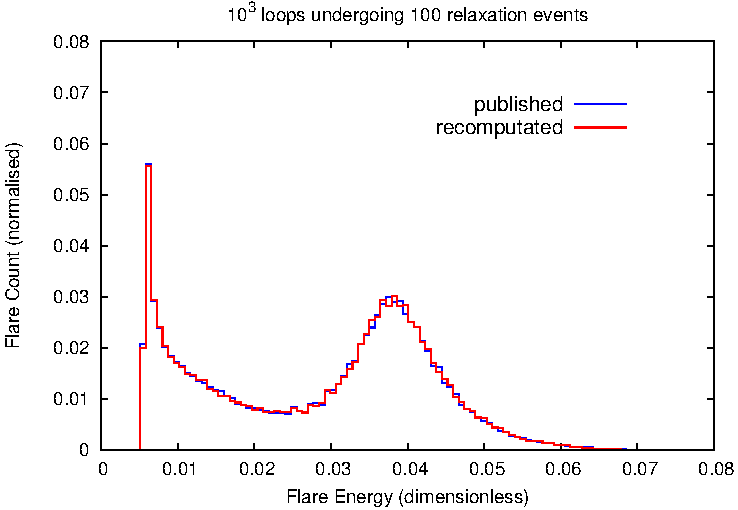
\includegraphics{../Group_3/wrpf_rx10e5_lle2}\\
  \vspace{5pt}
  %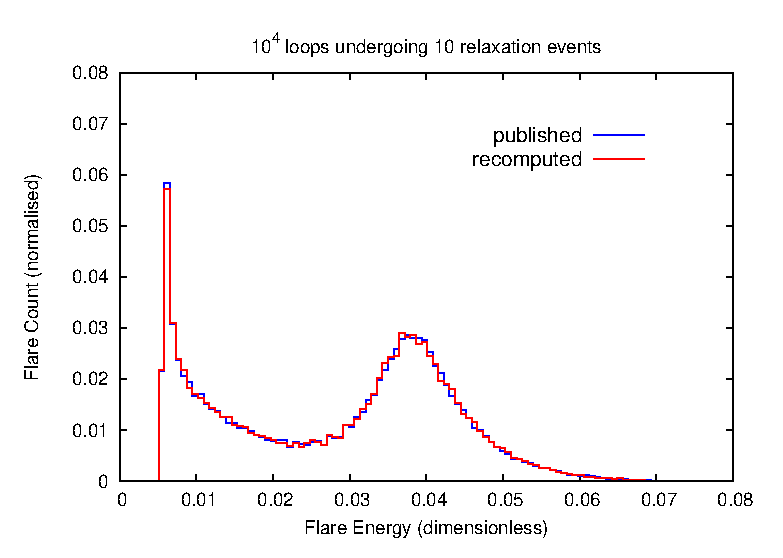
\includegraphics{../Group_3/wrpf_rx10e5_lle1}
  %\vspace{5pt}
  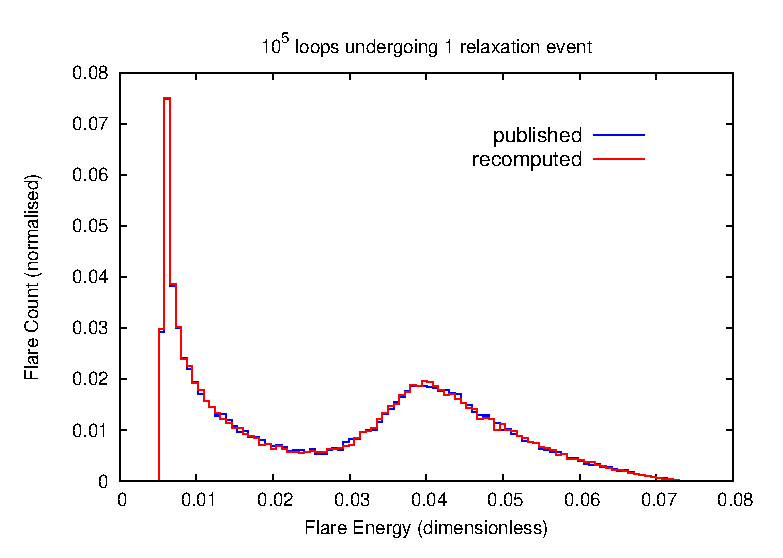
\includegraphics[scale=0.001]{../Group_3/wrpf_rx10e5_lle0}
  \caption{\small{Flare energy distributions over 10$^5$ relaxation events for two different loop lifetimes, 100 (top) and 1 (bottom) relaxation event(s). The red plots are the recomputed results and the blue are the results from the original paper \cite{bareford2010nanoflare}.}}
  \label{fig_recomp_grp3_exp2}
  %\vspace{-10pt}
\end{minipage} 
\end{figure}
The differences between the two sets of results are negligible and entirely consistent with the stochastic method used to generate the energy distributions.

\subsubsection*{Experiment 3: Atmospheric Physics}

For the third paper, we prepared pre-built software for reproducing 
  simulations of idealised atmospheric clouds presented in \cite{arabas2013libcloud}.
The paper covers description of an open-source C++ library named libcloudph++. 
The library is intended for representing microphysics of clouds and precipitation
  in numerical models -- coupling libcloudph++ with a fluid-dynamics solver 
  of an atmospheric flow allows one to study the formation of clouds and rain.

While the software has already been released under the open-source GPL license
  and has been accessible through a GitHub repository, there is still
  a potential legal issue.
The library features the implementation of an algorithm inspired by a technique 
  described in the scientific literature but also covered by several patents,
  including a European one (EP1847939A2). This prevents us from using the
  existing implementation.

Furthermore, the crux of the implementation is its support for execution
  on both CPUs and GPUs, the latter being optional but offering 
  significantly faster executions times.
However, the implementation uses the non-free CUDA standard what limits its potential
  users to owners of hardware of particular vendor and related proprietary software.

The only challenge in setting up the virtual machine was in providing all needed
  dependencies, namely recent versions of a C++ compiler, and the CMake, Boost and Thrust 
  packages.

\subsection{Discussion}

We encountered legal obstacles with all papers.
All of the software had been developed at universities, which typically results in the copyright being held by these institutions.
Furthermore, the decisions of whether to allow open-source distribution of the
code and the choice of licensing terms might be the prerogative of a university
representative (e.g.\ a PhD supervisor).
While this is in no way unique to non-CS domains, it is likely that pre-existing IP procedures are less likely to cover software dissemination aspects in institutions not dealing with computer science.
Even if the legal status of the code developed for a given experiment is settled and matches reproducibility requirements, the environment needed to run it might prevent unconstrained recomputation.
This in fact was also the case in one of the programs in question, as the code relied on a proprietary software library.

We also noted a lack of domain-specific workflows for recomputation in non-CS journals.
A counterexample is the Geoscientific Model Development (GMD) journal, which encourages reviewers to get
  acquainted with the code behind papers under review \cite{GMD_editorial_2013}.
Yet, the same journal, as of now, imposes a 50~MB limit on the size of electronic supplements 
  which effectively rules out shipping a VM together with the paper.

The level of computer proficiency in non-CS domains~\cite{Merali_2010} is also likely to influence the ability of researchers to use the virtual machines -- it is arguably less likely that a physics or urban-planning journal reviewer will be comfortable using a VM, in contrast to CS-related journals.
